\documentclass[12pt]{article}
\usepackage[spanish]{babel}
\usepackage{lingmacros}
\usepackage{tree-dvips}
\usepackage{amsmath, amsthm, amssymb}
\usepackage{graphicx}
\begin{document}


\title{Reporte: Accidentes de autos en Seattle}

\author{Carlos Ríos} 
\date{\small{\today}}

\maketitle


\section*{}
\subsection*{Por qué? (Introducción)}
Este trabajo esta dirijido para la sociedad en general y el objetivo es generar conciencia social respecto a los accidentes de trafico, por eso motivo el lenguaje será sencillo. Tomando en cuenta que los accidentes de tráfico representan la muerte de 1.3 millones de personas al rededor del mundo cada año (World Health Organization, en este trabajo se pretende comprender mejor este tipo de accidentes, y evaluar cuales son los factores más relevantes para que ocurran. Según The World Health Organization, las victimas (a nivel mundial) corresponde a transeuntes en un 50\% de los casos, también se explica que la mayoria de los accidentes en genera ocurren por errores humanos, sin embargo también existen factores ambientales, del automovil, o de las carreteras. Principalmente vamos usar Machine Learning para crear un modelo que clasifique los accidentes segun su nivel de severidad para poder predecir la probabilidad de un accidente segun nuevos features. \

\begin{figure}[htbp]
  \centering
    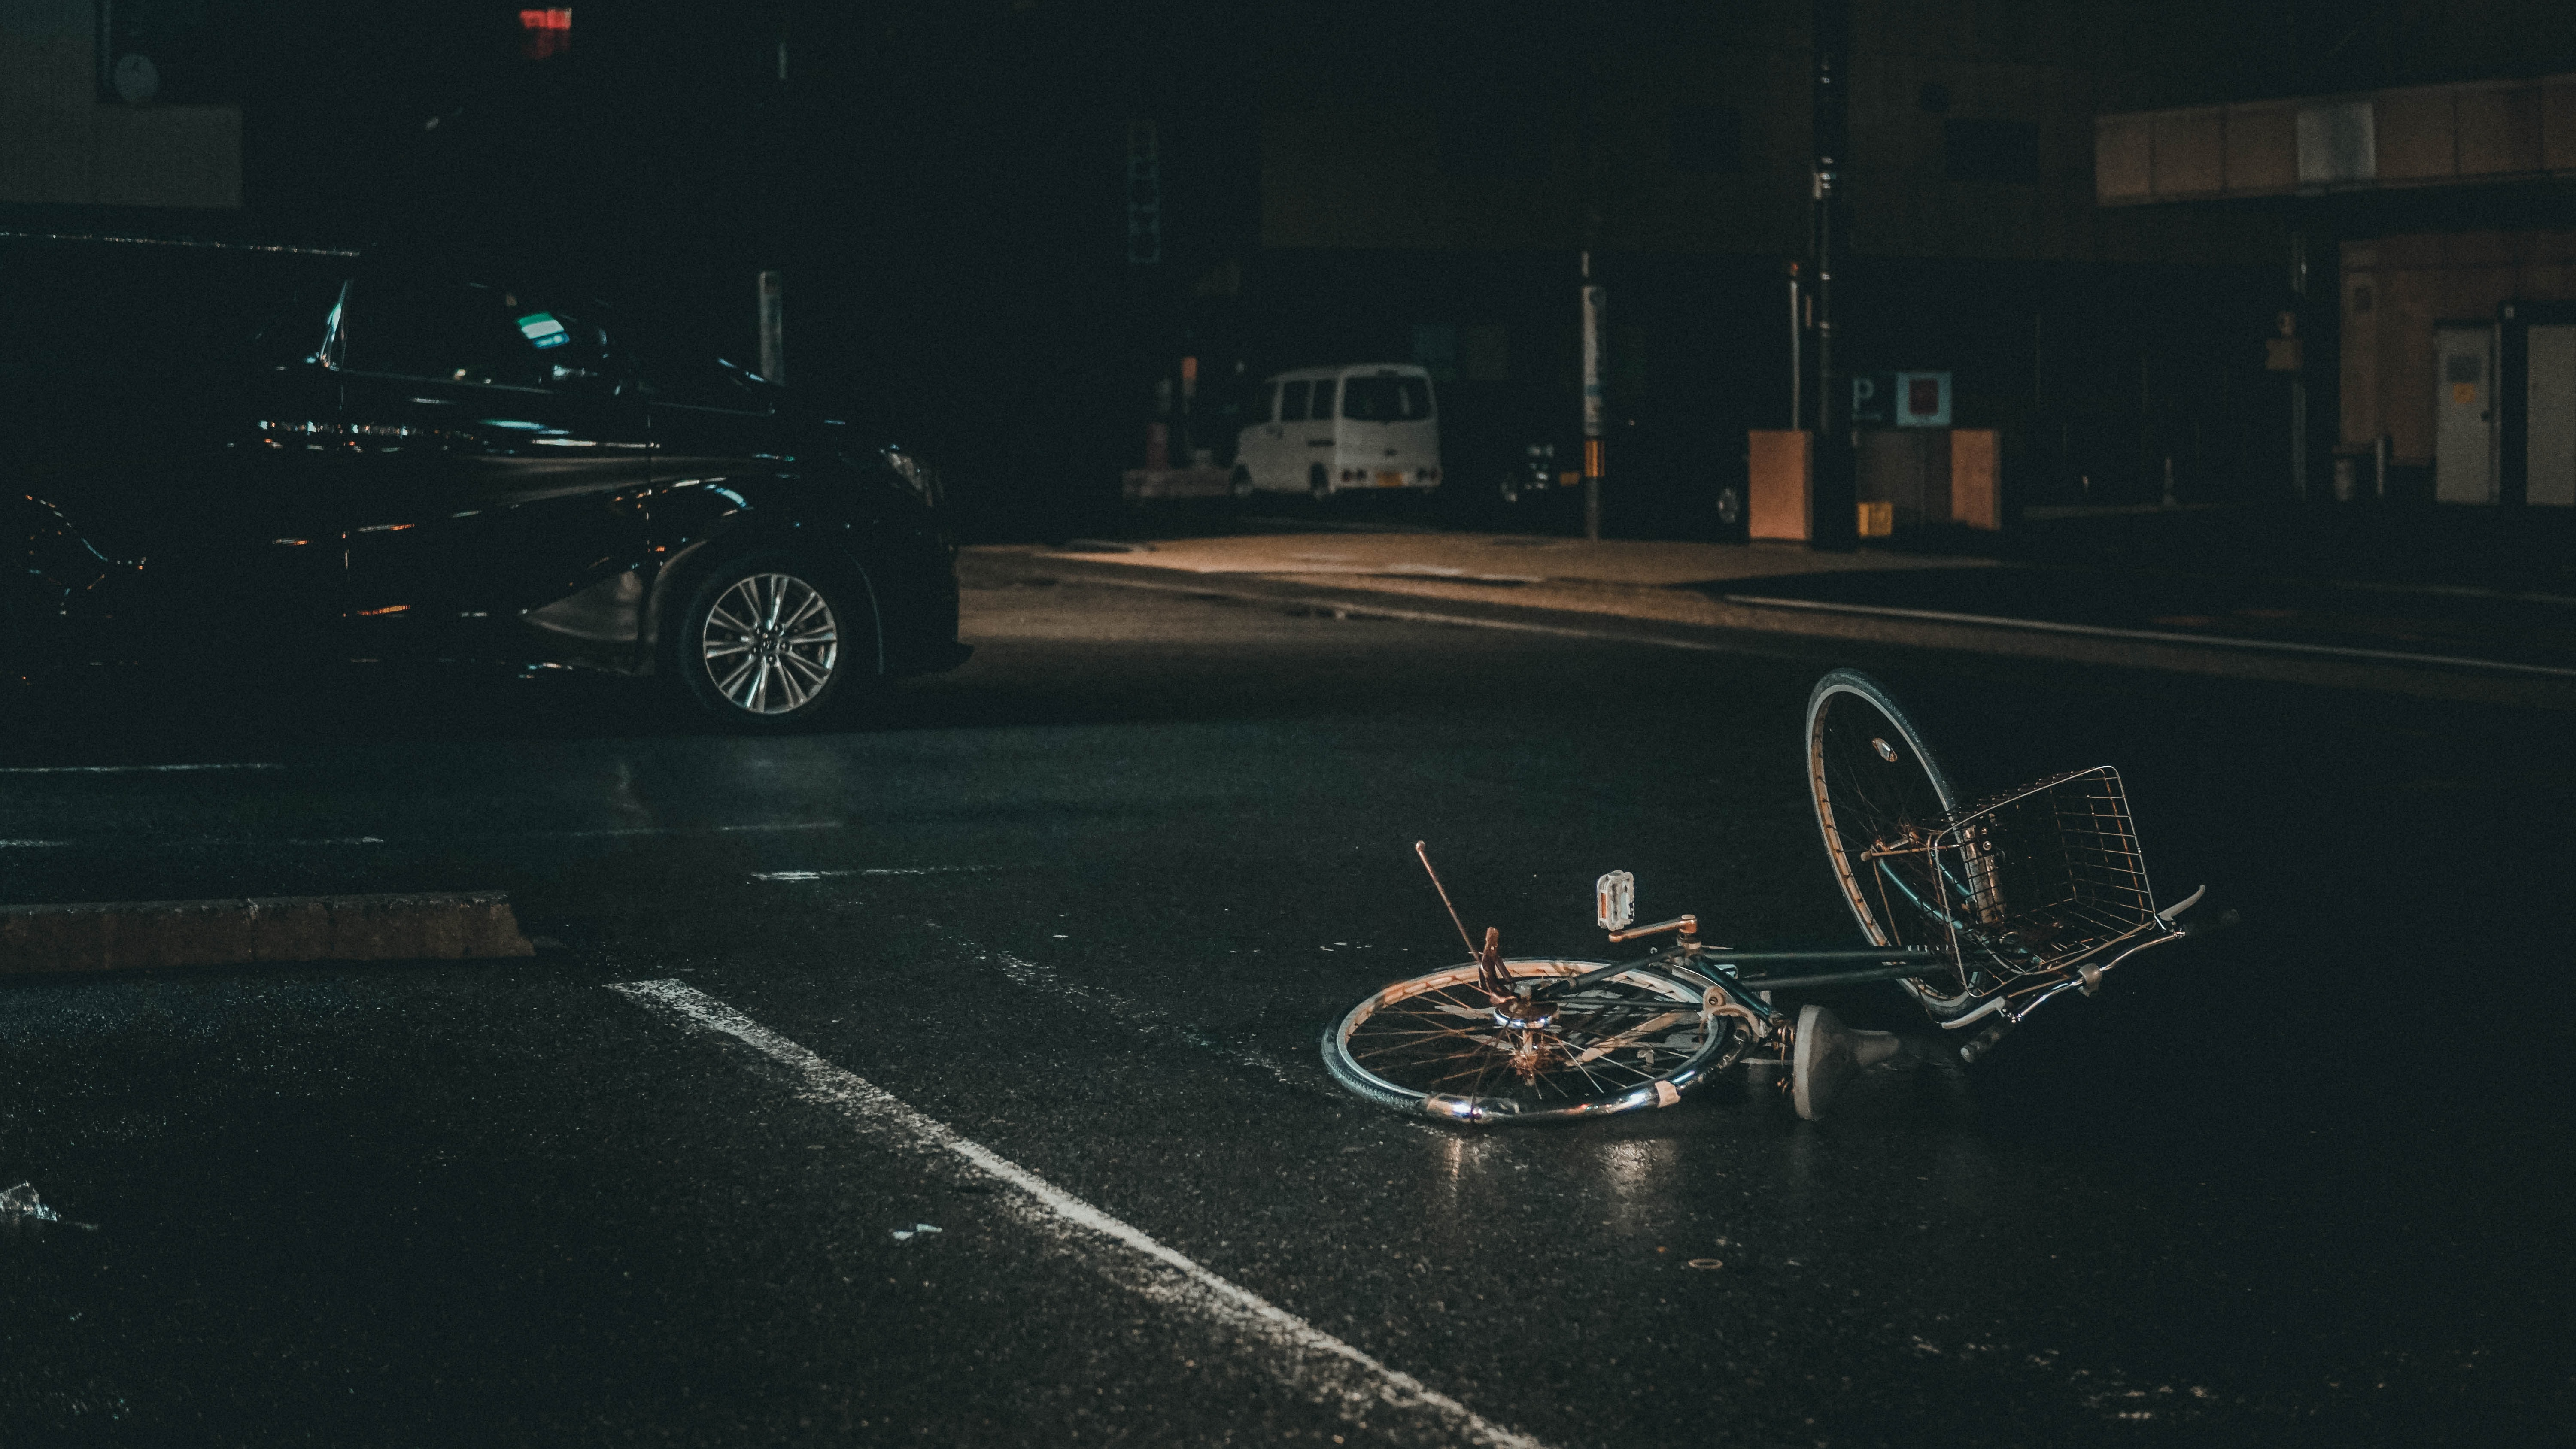
\includegraphics[width=1\textwidth]{../images/ian-valerio-9UxW_MqBGe4-unsplash.jpg}
  \caption{Photo by Ian Valerio on Unsplash.}
  \label{fig:intro}
\end{figure}




\subsection*{Sobre los datos}
Utilizaré la base de datos Collisions—All Years que nos provee SDOT Traffic Management Division de Seattle. Los datos estan conformados por 194673 casos, y contiene 38 features los cuales separaré en cuatro grupos:

a) Hay algunos features que no son relevantes para nuestro proposito por ejemplo aqullos que corresponden a codigos de identificación (id), también existen features repetidos o features con poca información. 

b) Existen features que quizas no son relevantes para aplicar técnicas de machine learning pero que si lo son para comprender mejor el problema, por ejemplo la ubicación, las coordenadas y la fecha. 

c) Por otro lado estan aquellos features que muy probablemente tengan una fuerte influencia sobre la severidad del accidente. Incluso estos hay que trabajarlos porque muchos contienen un codigo numerico que no se refiere a un valor numerico sino es un codigo de identificación para cierto tipo de accidente. Por ese motivo es necesario usar label encoder o un one hot encoder. Entre ellos estan:\\
\textbf{SEVERITYCODE} Esta es la etiqueta de clasificación de choques, es el feature que nos servirá para clasificar los choques en: 1) Sólo daños de propiedad o 2) Colisiones con heridos. \\
\textbf{ADDRTYPE} Es el tipo de calle en la que se encontraba: Block, intersection or Alley.\\
\textbf{COLLISIONTYPE} Es el tipo de colisión. \\
\textbf{PERSONCOUNT} Es la cantidad de personas involucradas en la colisión.\\
\textbf{PEDCOUNT} Es la cantidad de transeuntes involucrados. \\
\textbf{PEDCYLCOUNT} Es la cantidad de ciclistas involucrados en la colisión.\\
\textbf{VEHCOUNT} Es la cantidad de vehiculos involucrados en la colisión.\\
\textbf{JUNCTIONTYPE} Es el tipo de empalme.\\
\textbf{UNDERINFL} Si la persona esta bajo algun influencia alcoholica o narcótica.\\
\textbf{WEATHER} Es el clima.\\
\textbf{ROADCOND} Es la condición en la que se e contraba el camino.\\
\textbf{LIGHTCOND} Describe el tipo de luz que habia durante la colisión.\\
\textbf{SDOT COLCODE} Es un codigo de SDOT que describe la colisión.\\

\subsection*{Metodología y resultados}
Explicare la metodología y los resultados en un solo subtitulo pues desarrollaré en incisos cada parte.

 Los primeros analisis exploratoríos fueron, principalmente, contar casos para cada variable, se econtró por ejemplo que en la mayoria de accidentes estan involucradas dos personas. Mostraré los resultados más interesantes que encontré, mediante histogramas. 


     Se hicieron lo siguientes analisis: 1) Analizar la cantidad de accidentes de tráfico año a año. 2) Determinar los días en los que ocurren más accidentes y en cuales menos. 3) Cómo se distribuyen los accidentes en la ciudad. 4) Qué tipo de colisiones son las qué más ocurren? Cuáles son las que dejan más heridos? 5) Describir mediante un arbol de descición qué factores son relevantes para que haya heridos en un accidente de tráfico? \\

     1) Se contabilizaron la cantidad de accidentes año a año desde el 2004 hasta el 2020. Se puede observar que año a año hay un descenso de accidentes, a excepción del año 2015 en el que hay un pico de daños a la propiedad. En promedio cada año se producen 3590 accidentes con heridos y 8447 accidentes sólo de daños a la propiedad. En estos valores medios se omitieron los años 2004 y 2020 pues no se tiene registro de los años completos, fig. \ref{fig:years}. \\

      

  \begin{figure}[htbp]
    \centering
      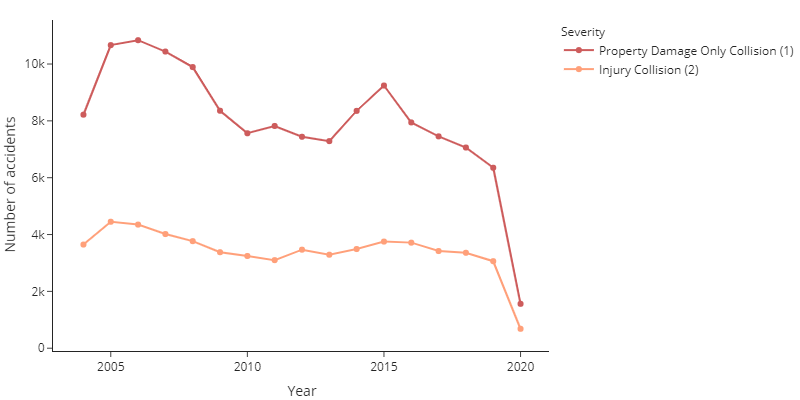
\includegraphics[width=1\textwidth]{../images/years.png}
    \caption{Accidentes de automoviles año a año desde el 2004 hasta el 2020.}
    \label{fig:years}
  \end{figure}


2) También se contabilizaron los días en los que ocurren más accidentes.  Sin duda los días en los que más occurren los accidentes son los días viernes, a diferencia de los días domingos en los que occurrieron un 20\% menos de accidentes, fig. \ref{fig:dayofweek}. \\
\begin{figure}[htbp]
    \centering
      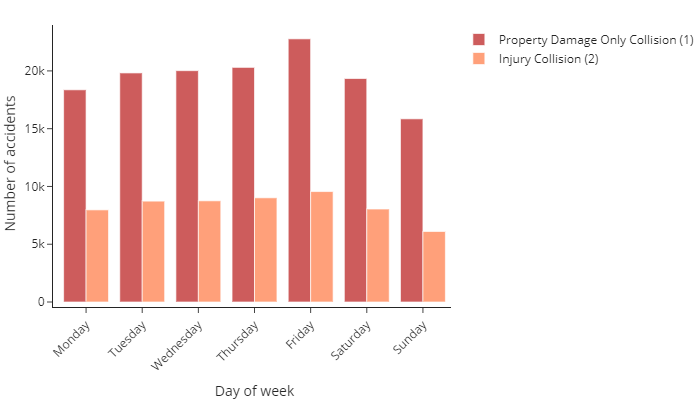
\includegraphics[width=1\textwidth]{../images/day_of_week.png}
    \caption{Histograma de accidentes de automoviles por día de semana.}
    \label{fig:dayofweek}
  \end{figure}
  
  3) La distribución geoespacial nos brinda una una mejor comprensión de los accidentes, fig. \ref{fig:map}. Como se puede observar esta es una visualización de 7000 registros obtenidos entre el año 2004 y 2020 de accidentes en Seattle (aunque se cuentan con más de 19000 registros, el computo es bastante pesado). El siguiente grafico muestra cómo estan distribuidos los accidentes y por la forma de las calles puedo inferir que en el centro urbano de la ciudad ocurren muchos más accidentes que en los suburbios.\\

  \begin{figure}[htbp]
    \centering
      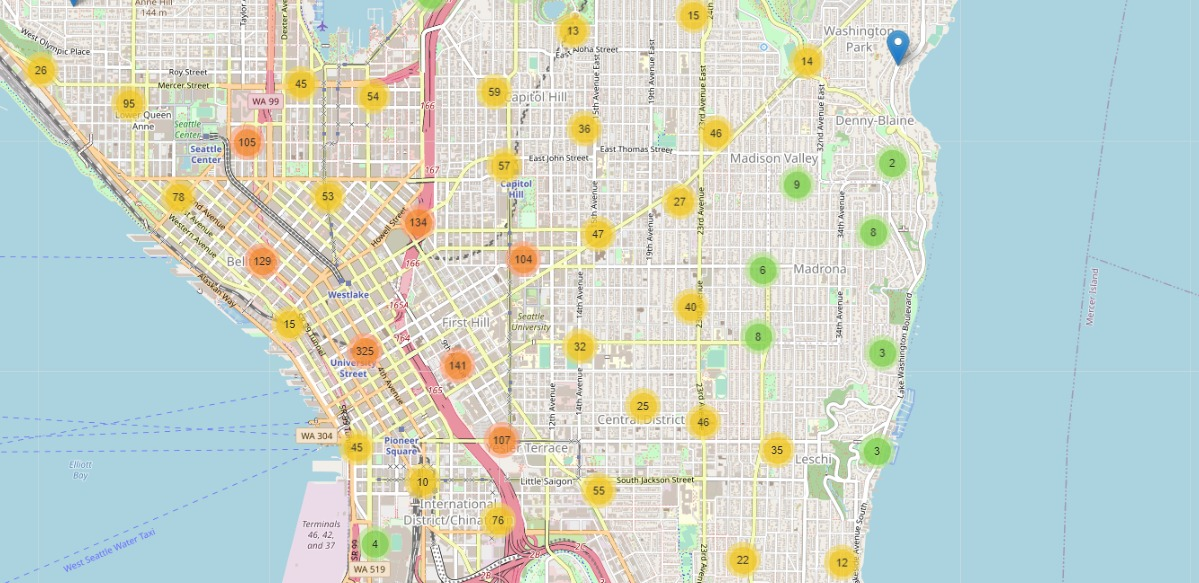
\includegraphics[width=1\textwidth]{../images/map_d.jpeg}
    \caption{Mapa de Seattle con los accidentes de automoviles. Este mapa se generó tan solo con 7000 datos. }
    \label{fig:map}
  \end{figure}



  4) Al contabilizar los tipos de colisiones encontramos que sin duda la mayoria de las veces que solo hay daños materiales es por que el automovil estaba parqueado. Sin enmbargo, los accidentes con heridos se producen principalmente porque la colisión fué en angulo o porque el automovil fue chocado por atras, fig. \ref{fig:collitiotype}. 

  Me pareció sumamente curioso la asimetria entre la cantidad de choques del tipo girar a la derecha en comparación a girar a la izquierda. Pude conversar con un conductor de camiones que recorrio la mayoria de las carreteras de EEUU y el me explicó que se podía deber a que cuando uno gira a la derecha solo se involucra un carril, mientras que cuando uno gira a la izquierda intervienen 3 carriles (el de sentido opuesto, el transversal y el de sentido opuesto al transversal) entonces por eso motivo ocurren muchos más accidentes girando hacia la izquierda que hacia la derecha. Aunque otro posible explicación es son los puntos ciegos que los automoviles tienen por su misma fabricación. \\


  \begin{figure}[htbp]
    \centering
      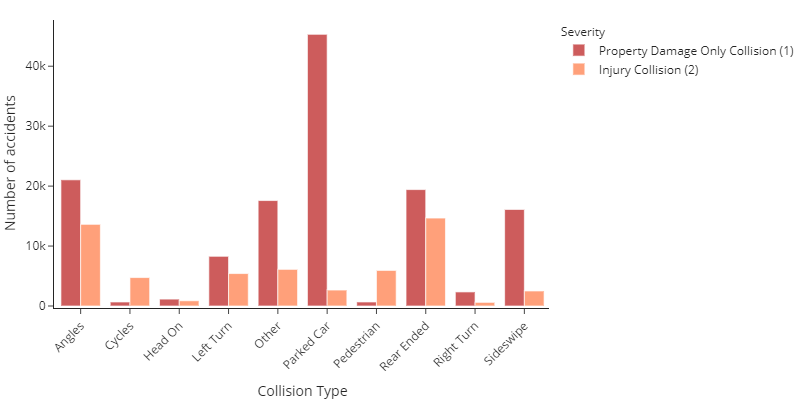
\includegraphics[width=1\textwidth]{../images/collition_type.png}
    \caption{Cantidad de de accidentes por tipo de colisión}
    \label{fig:collitiotype}
  \end{figure}
  5) Antes de analizar el arbol cabe decir que las variables estaban muy levemente correlacionadas, es decir no habia una clara relación entre cual era el factor más descisivo para que se produzca una colisión con heridos o solo de daños materiales.  El árbol tiene un accuracy de 0.64 que sin duda es mejorable, fig. \ref{fig:tree}.

  Lo que nos quiere decir este árbol es que si no hay ciclistas, ni transeuntes lo más probable es que sólo sean daños materiales. Mientras que dependiendo del tiepo de colisión, las luces o el tipo de junción, hay más probabilidad de que hayan accidentes con heridos. Por el lado derecho, nos dice que si la cantidad de personas es mayor a 6.5 y la cantidad de vehiculos involucrados es mayor a 2.5 hay una alta probabilidad de que en el choque hayan heridos.\\

  \begin{figure}[htbp]
    \centering
      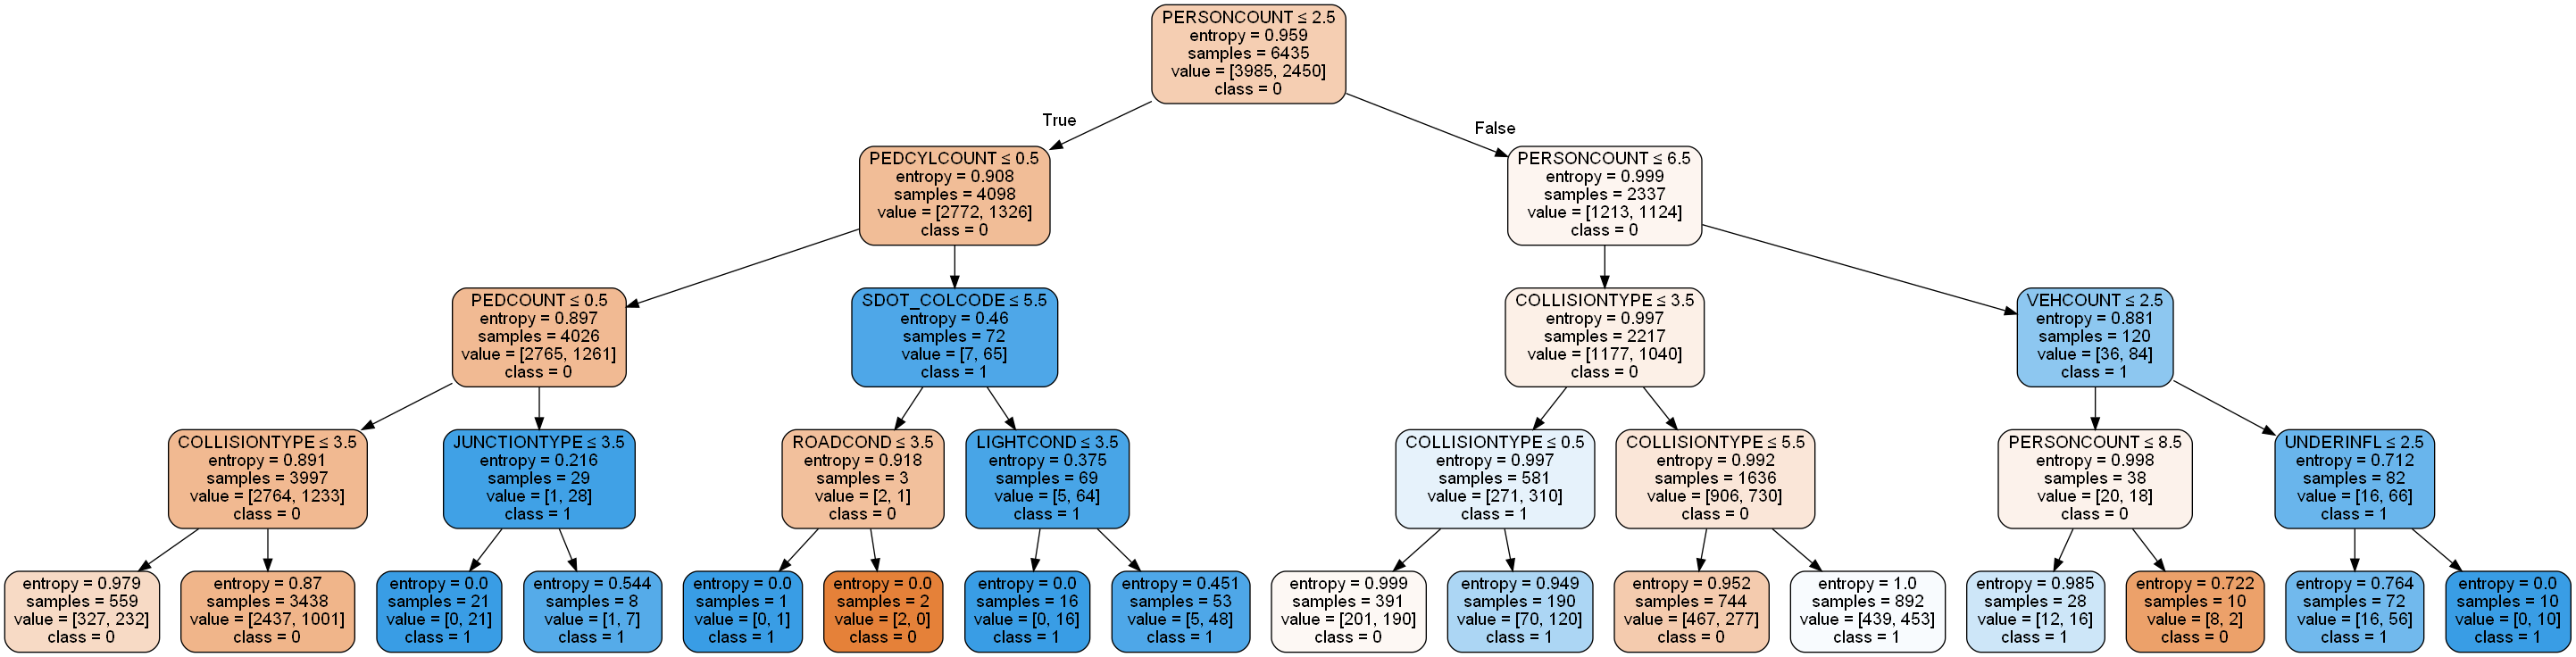
\includegraphics[width=1.5\textwidth, height=0.63\textwidth, angle=90]{../images/tree1.png}
    \caption{Árbol de descición utilizando los parametros más relevantes.}
    \label{fig:tree}
  \end{figure}

  \subsection*{Conclusiones}

  Sin duda el árbol se podria mejorar con un mejor entendimiento de los features así podriamos tener un label encoder más acorde. 

  Por otro lado mi sugerencia es que seas más precavido los días viernes, no dejes tu auto parqueado en cualquier lado, sé más precavido cuando conduzcas por el centro y por último fijate bien cuando gires a la izquierda!

  \subsection*{Agradecimientos}
  Victor Once - Comercial Driver. 
\end{document}